%
% File naaclhlt2016.tex
%

\documentclass[11pt,letterpaper]{article}
\usepackage{naaclhlt2016}
\usepackage{times}
\usepackage{latexsym}
\usepackage{hyperref}
\usepackage{graphicx}
\naaclfinalcopy % Uncomment this line for the final submission
%\def\naaclpaperid{***} %  Enter the naacl Paper ID here

% To expand the titlebox for more authors, uncomment
% below and set accordingly.
\addtolength\titlebox{.5in}    

\newcommand\BibTeX{B{\sc ib}\TeX}

%
\title{Menu Price Prediction using Neural Netwokrs}

% Author information can be set in various styles:
% For several authors from the same institution:
% \author{Author 1 \and ... \and Author n \\
%         Address line \\ ... \\ Address line}
% if the names do not fit well on one line use
%         Author 1 \\ {\bf Author 2} \\ ... \\ {\bf Author n} \\
% For authors from different institutions:
% \author{Author 1 \\ Address line \\  ... \\ Address line
%         \And  ... \And
%         Author n \\ Address line \\ ... \\ Address line}
% To start a seperate ``row'' of authors use \AND, as in
% \author{Author 1 \\ Address line \\  ... \\ Address line
%         \AND
%         Author 2 \\ Address line \\ ... \\ Address line \And
%         Author 3 \\ Address line \\ ... \\ Address line}
% If the title and author information does not fit in the area allocated,
% place \setlength\titlebox{<new height>} right after
% at the top, where <new height> can be something larger than 2.25in
\author{Michele Ceru \\
	    Center for Data Science\\
		New York University\\
	    {\tt mc3784@nyu.edu}
	  \And
	Luisa Quispe Ortiz\\
  	Center for Data Science \\
  	New York University\\
  {\tt lqo202@nyu.edu}}

\date{}

\begin{document}

\maketitle

\begin{abstract}
Culture diversity and socioeconomical groups strenghten are marked by the way language is used in each of them.
Many studies have shown that there is a relation between how a restaurant describes itself and price a restaurant charge (or the price range it has), based on the previous statement. Therefore, it may be possible to find use menu's description to predict the price of a dish. We aim  to perform this task taking advantage of tools such as word embeddings and neural networks, that we believe will aide and facilitate the objective.
\end{abstract}

\section{Introduction}

NYC known as being a city that has influence of several cultures, its cuisine reflects that too. Across all the city it is possible to find chinese, italian, mexican and many more kitchen’s of the world having a myriad of plates and prices.

Many factors influence the price, from external sources such as inflation, availability, critic’s reviews and even customer opinions \cite{jurafsky2014language}; to internal preferences of the restaurant owner such as location, stuff, etc. 

Each restaurant knows their target customer, hence all the business is focused on that, this includes the menus. This implies a relation between socioeconomic class and language \cite{freedman2011authenticity}, which is also considerd to be Bordieu's distinction \cite{jurafsky2016bordieu}. Therefore, there is evidence of a relation between how a restaurant describes its plates and how much it charges. It may be possible to predict the price of a dish given the description of it. 

There are some previous works that are related to the mentioned task, some of them from a economics point of view, others from a culinary approach and a few from a linguistics one. Their objective vary according to the approach taken. For example, in economics it was important to see the impacts of reviews on sells, while in culinary and hospilatity the objective is to language used in the menus mainly to make recommendations for writing \cite{chahuneau2012word}.

Although, some handful insights were found such as in \cite{chahuneau2012word,jurafsky2014language,jurafsky2016bordieu}: 5-stars restaurant tend to use more fancy words and borrow expressions from other languages, while the chinesse restaurant have a wider variety of food and tends to use just a small phrase to describe its plates. 

None of the previous literature, however, used distributed word representations and neural networks to predict the menu's price. Using word representations will aide to understand the underlying semantic relation between words \cite{mikolov2013efficient} in the culinary aspect. And training using neural networks will bring us the possibility of capturing non-linear relationships between the embeddings and the target variable price \cite{}, even more if we consider the word order as in recurrent neural networks (LSTM or GRU). We believe that by using these tools, we will find and confirm some conclusion other studies have had, which will  result in an improvement of the error indicator. 


\section{Prior Literature}

As stated in \cite{chahuneau2012word}, most of the previous works are in the linguistics, hospitality research and economics fields. Each of them gives a slightly different approach, given that they aim to explain distinct points of view. However, it's good to have a starting point.

Socieconomic groups are defined by the way they use the language, this is widely known and used by politicians. In \cite{freedman2011authenticity}, the authors claim that the previous phrase is true, even more, they assert that food is a "robust marker of group identity" too. They show that prices affect the language in food advertising, specifically in potato chip bags. 

There has been also works in prediction using text, such as the one described in \cite{archak2011deriving} where they analyze the impact of reviews on product sales, a marketing and economics point of view. They focus on a couple of products and identify "beliefs" a customer has in a feature of the product, not considering a polarized review (positive or negative based on the rating). This has not been the only prediction task using text that can be found, in fact \cite{chahuneau2012word} mentions examples of predicting risk in financial markets and based on reviews (also movies) to other several economic tasks. 

In the field of culinary and hospitality research, there are many manuals that have recommendations for writing menu descriptions, according to \cite{chahuneau2012word} and \cite{jurafsky2014language}, such as \cite{kasavana1990menu} . Actually is interesting to notice that by conducting an experiment in a small cafeteria \cite{wansink2005descriptive} showed that the menu description does affect the customer's behavior and perception.

The logic that menu's descriptions produce change considering the restaurant's niche (public they are directed to), and the fact that this follows linguistic socieconomical differentiation, is mentioned and explained in the first chapter of \cite{jurafsky2014language}, where he cites a myriad of works and their main implications in the relationship between prices and descriptions. Jurafsky assures that expensive restaurants' menus tend to use "native" words borrowed from other languages such as french, italian, spanish, use fancy words in long descriptions and they also focus more in the detail of the description and avoid using filler words. On the other hand, common restaurants have a wider variety of plates, for they will try to sell them by describing in a simple and shorter way that may use a lot of filler words ("real cream cheese", "home-baked cookies"). 

Our main article is  \cite{chahuneau2012word}, as one its goals is to predict the price and how it is influenced by  the use of language. The article uses menu descriptions from main cities across the U.S. as well as some descriptive features extracted from Yelp reviews (flag variables of wi-fi, parking, delivery, etc), as these were also used to do sentiment analysis. Their analysis is mainly linguistical, as they wish to know how each word or change of word affects the price, using regression tools.


In a more recent background, a study  \cite{jurafsky2016bordieu} focus on the study the reflections of Bourdieu's distinction, which happens to consider that there are deep associations linking food culture with social class and other aspects of identity, using the language of food. They split their study in 4 aspects, that define the relation between food and social culture. Using Yelp reviews they conclude that words used in menu descriptions reflect the many aspects of Bourdieu's distinction. In general terms, these distinctions are mainly the ones mentioned in the previous paragraph with a couple of new hypothesis, so the study is kind of confirmatory.

\section{Data}
To gather the information required by the project, and considering previous works data, we crawled AllMenus.com (\url{www.allmenus.com}). Initially we only got New York City menus, but to ensure consistency in our results by having a larger sample, we decided to also consider San Francisco. We ended up with 467,669 NY menu descriptions and 200,020 from SF. For us, each of these rows is a observational instance, as we will only model with the text in each row. So, the features captured were: restaurant name,  section of the menu, subsection of the menu, dish name, dish price and description, from which we will take the price as our target and the dish name and description as our input text.

Before moving on the modeling task, we made a quick analysis of our information in order to detect any anormality.  The first we could find is that only 99 observations had null price which we set to zero price, the rest was encoded in different ways, but it was possible to obtain the price value of the plate. 

Then, we wanted to see the distributions per city, and whether there was significant difference that pointed us to do separately analysis. The mean price of SF is of \$9.77, one more dollar than the mean of NYC, a similar relation was found in the medians as NYC's was of \$6.99 against \$7.99 in SF. Despite this, by looking at the normalized (standardized) distributions in Figure \ref{fig:price_dist}it was possible to see that both seemed alike, highly skewed. 

   \begin{figure}[thpb]
      \centering
      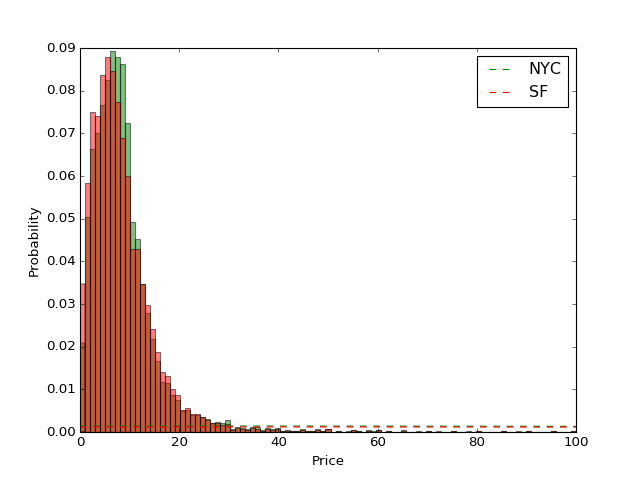
\includegraphics[width=6cm, height=4cm]{dist_sf_nyc_prices}
      \caption{Distribution of the prices in NYC and SF}
      \label{fig:price_dist}
   \end{figure}

This gave us evidence to keep on analyzing all the dataset together. 

In the text, we made a tokenizer that deleted some punctuation signs and that lower case all the input.

For all our runs, the whole set of restaurants item's price was split into training(80\%), validation (10\%) and testing(10\%) set randomly, considering that the proportion of observations per city will maintain due to randomness. 

\section{Modeling Framework}
Before explaining our protocol, we give some brief definitions about the tools that will be used.
\subsection{Word Embedding}
Distributed representation of words widely used nowadays, they are just ubiquitous to NLP, as they provide semantic relation between words \cite{hill2016learning}.  A good example is the known \textbf{Word2Vec} experiment from Google's team, in which they were able to collect semantic relationships between words using a large corpora (private) to first predict the word that is in the middle of other 3 known as Continuous Bag of Words and the reverse process, to predict the words around a specific one known as Skip-gram. \cite{mikolov2013distributed,mikolov2013efficient}

\subsection{Neural Netwokrs}

\subsection{ Protocol}

\section{Results}
\section{Analysis}
\section{Conclusions}
\section*{Acknowledgments}

\section*{Collaboration Statement}


\bibliography{naaclhlt2016}
\bibliographystyle{naaclhlt2016}



\end{document}